
In this section, we will provide examples of the applications of TDA methods in machine learning. We provide four examples from published papers and outline their model and how they applied TDA in their project.

\subsection{PH for Point Clouds: Shape Recognition} \label{sec:shape}
\begin{wrapfigure}{r}{3in}
\vspace{-.2in}
\centering
    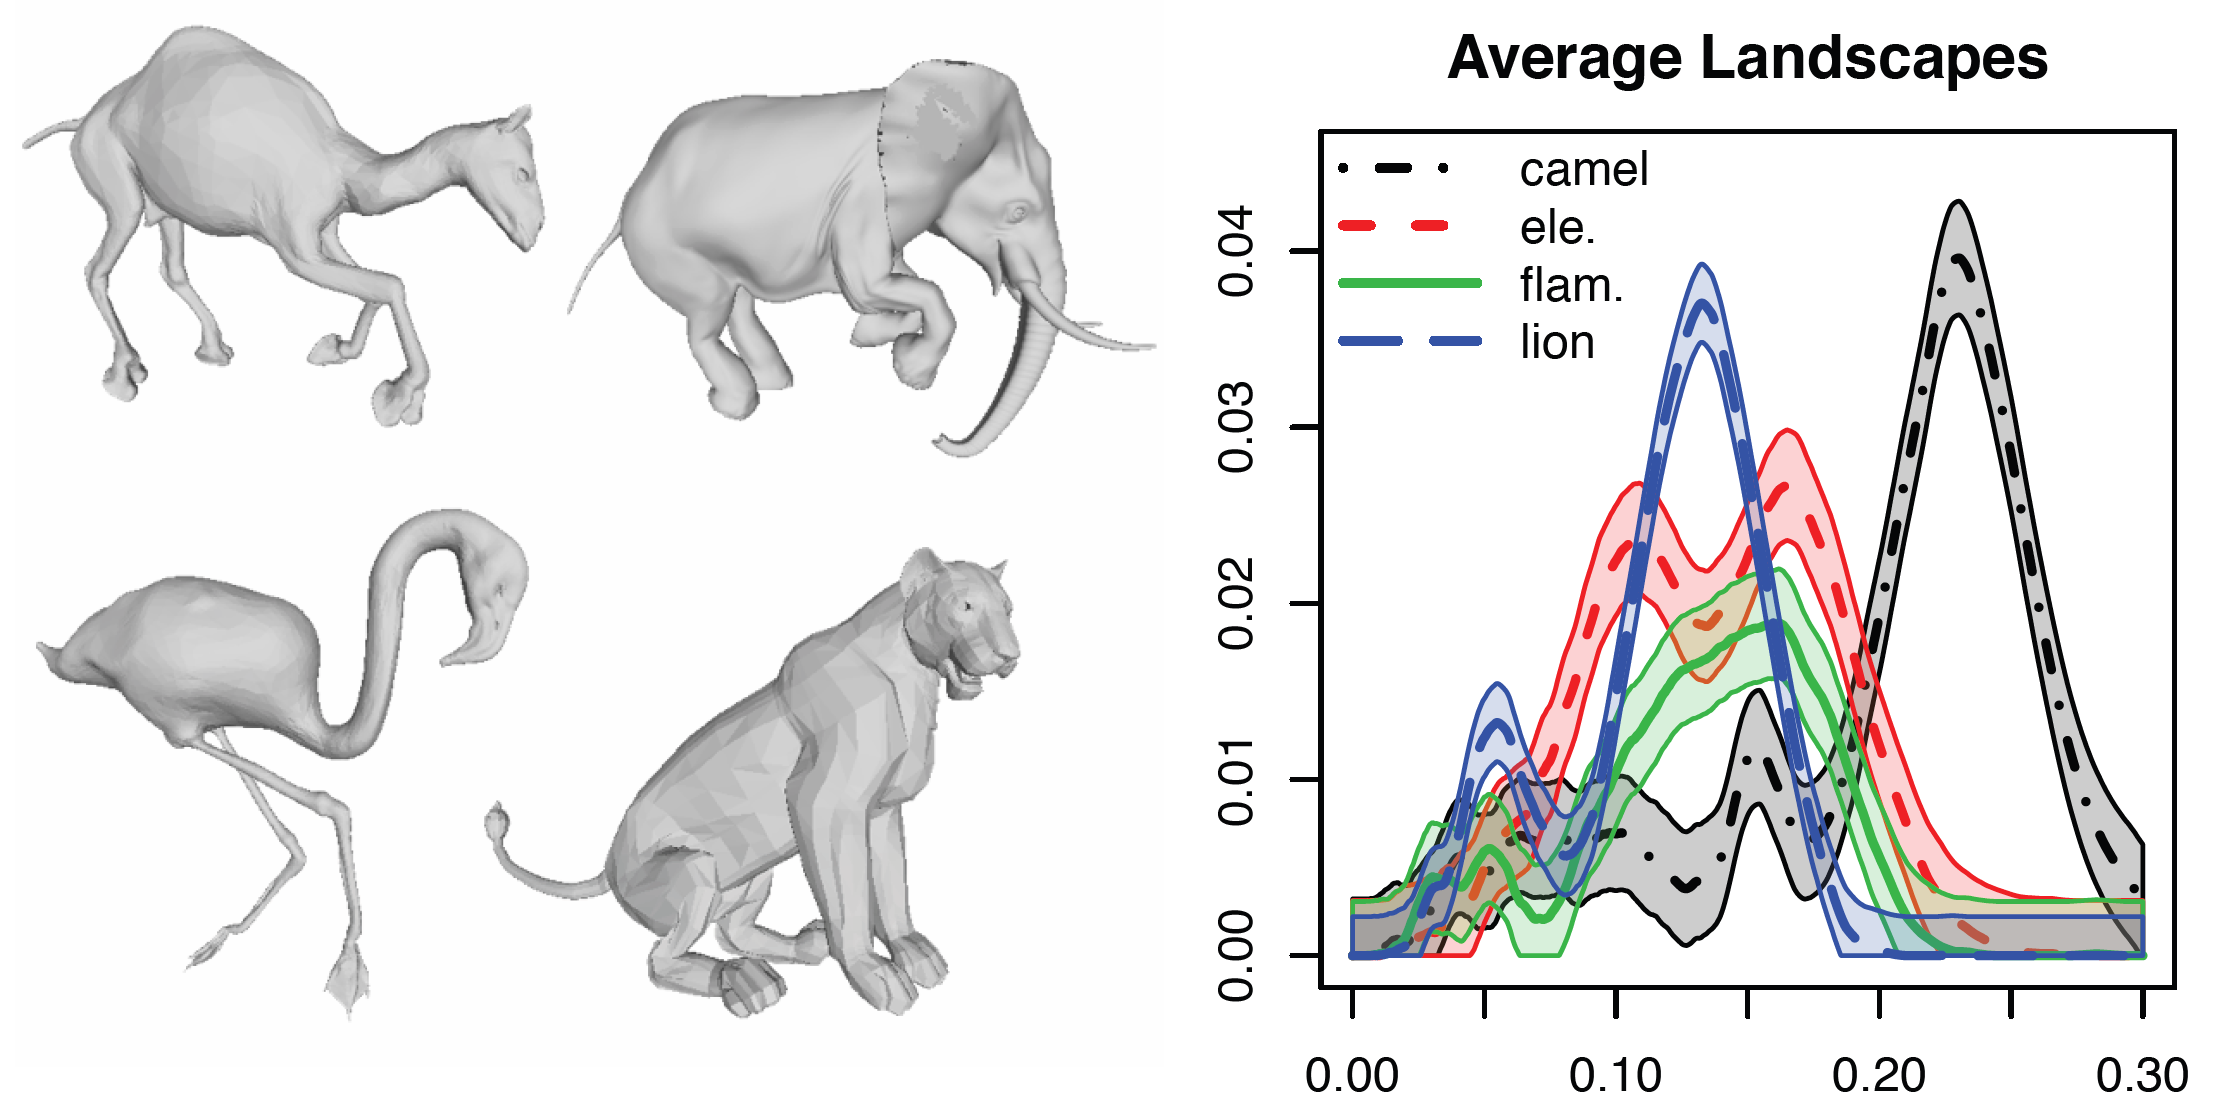
\includegraphics[width=\linewidth]{figures/shape-recognition-example.png}
    \caption{\footnotesize  {\bf Shape Recognition via PH.} In \cite{chazal2015subsampling}, the authors obtained 100 point clouds for each animal by subsampling the surfaces above and analyzed their persistence landscapes. On the right, they present the 95\% confidence bands for the persistence landscapes of these 400 point clouds, demonstrating that each animal's persistence landscape exhibits significantly distinct characteristics. The figure is adapted from~\cite{chazal2015subsampling}. \label{fig:shape}    }
    \vspace{-.2in}
\end{wrapfigure}
In this section, we present an illustrative example of the utilization of PH in shape recognition, based on the work~\cite{chazal2015subsampling}, where Chazal et al. demonstrated the effectiveness of PH in shape recognition. One specific example involved four different animals: an elephant, flamingo, lion, and camel, each representing a unique shape in $\R^3$, where each shape is normalized to have a diameter of one. They began by selecting 500 random points from the surface of each animal, as shown in~\Cref{fig:shape}, resulting in the point clouds $\X_E$, $\X_L$, $\X_F$, and $\X_C$ for the elephant, lion, flamingo, and camel, respectively. Then, they created 100 subsamples of 300 points each from these point clouds, resulting in 400 different point clouds: $E_i \subset \mathcal{X}_E$, $L_i \subset \mathcal{X}_L$, $F_i \subset \mathcal{X}_F$, and $C_i \subset \mathcal{X}_C$ for $1 \leq i \leq 100$.

 

Next, they performed Rips filtration on each point cloud $\{E_i,L_i,F_i,C_i\}_{i=1}^{100}$ (see \Cref{sec:point_cloud}) and computed the corresponding persistence diagrams for dimension one. By vectorizing these persistence diagrams, they obtained the persistence landscapes for each point cloud, resulting in 400 persistence landscape functions: 
$\{\lambda(E_i), \lambda(L_i), \lambda(F_i),  \lambda(C_i)\}_{i=1}^{100}$.
In~\Cref{fig:shape}, they present the 95\% confidence bands for the true average landscapes (bold curves) of each class. e.g., blue confidence band correspond to 100  persistence landscapes coming from lion point clouds $\{\lambda(L_1), \dots, \lambda(L_{100})\}$. The narrowness of these confidence bands indicates that PH techniques provide robust shape-embedding methods that are minimally affected by noise. Moreover, the distinct confidence bands for each class underscore the effectiveness of PH in shape recognition. We also note that recent work by T\"urke\c{s} et al.~\cite{turkes2022effectiveness} studied the effectiveness of PH for shape recognition in different settings.




\subsection{PH for Graphs: Crypto-Token Anomaly Forecasting} \label{sec:crypto}

Three primary types of problems dominate graph representation learning: graph classification, node classification, and link prediction, as outlined by Hamilton et al.~\cite{hamilton2017representation}. These tasks encompass a broad range of real-life applications, including brain connectivity networks, molecular property prediction, recommender systems, fraud detection and transaction networks. In a related study, Li et al.~\cite{li2020dissecting} employ persistent homology to extract effective feature vectors from weighted and directed Ethereum crypto-token networks, modeled as temporal graphs. The approach is tailored for graph anomaly prediction, a specialized form of graph classification.  
 

 



The research problem is set as a prediction task where the authors aim to predict whether the absolute price return of an Ethereum token will change significantly beyond a predefined threshold $ |\delta| > 0 $ within the next $ h $ days. This involves analyzing the token's transaction network and its price fluctuations over multiple discrete time graph snapshots. The price information is sourced from external ground truth data, as token prices are determined by trading on blockchain exchanges.

For each snapshot, the authors use transferred token amounts on edges to define distances between adjacent vertices. These functions help  establish the similarity between nodes:
$\omega_{uv} = \left[1 + \alpha \cdot \frac{A_{uv} - A_{min}}{A_{max} - A_{min}}\right]^{-1}$ 
where $ A_{uv} $ represents the amount of tokens transferred between nodes $ u $ and $ v $, and $ A_{min} $ and $ A_{max} $ are the minimum and maximum transferred amounts, respectively. The authors set the parameter $\alpha = 9$ to map these weights to the interval $[0.1, 1]$, thus standardizing the weight values.
 

\begin{wrapfigure}{r}{3in}
\vspace{-.2in}
    \centering
	\subfloat[\footnotesize Tronix \label{fig:tronix}]{
        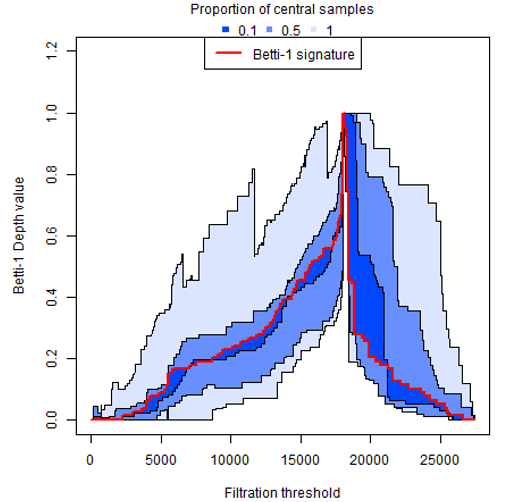
\includegraphics[width=.48\linewidth]{figures/5tronixB1_trim.png}}
	\subfloat[\footnotesize Power Ledger \label{fig:power_ledger}]{
        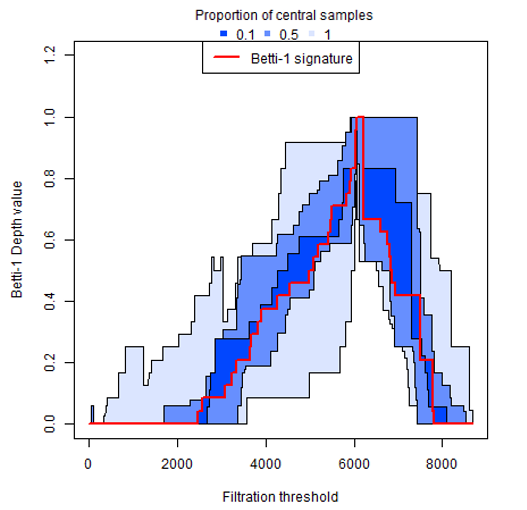
\includegraphics[width=.5\linewidth]{figures/5powerledgerB1_trim.png}}
    \caption{\footnotesize {\bf Betti pivots.} Comparative functional summaries of the Tronix and Power Ledger token networks over seven days, displaying daily Betti-1 values across various scaling parameters. Each plot captures the evolution of topological features, with the central red lines indicating the Betti pivots. These pivots represent the most stable or 'normal' network structures, providing insights into network behavior and potential anomalies driven by underlying transaction activities. The figure is adapted from~\cite{li2020dissecting}.}
    \label{fig:mbd}
 \vspace{-.1in}
\end{wrapfigure}
By treating the edge weights (similarity measures) as distances between nodes, i.e., \( d(u,v) = \omega_{uv} \), the authors construct a filtration of Rips complexes (\Cref{sec:graph}-ii) from the snapshot graphs. For non-adjacent nodes, the distance is defined by the shortest path in the graph. The main insight here is to extract topological patterns developed in the graphs at multiple scales. This process involves forming a simplicial complex where nodes are connected if their distance is within a threshold \( \epsilon \), reflecting their similarity based on the edge weights. Essentially, nodes with high similarity (those with large transaction amounts between them) are connected early in the filtration, while more distant nodes appear later. 

The authors then compute persistence diagrams from these filtrations and convert them into Betti functions. Additionally, they introduce new functional summaries of topological descriptors, namely Betti limits and Betti pivots, which track the evolution of topological features as the scale parameter \( \epsilon \) changes over the snapshots. \Cref{fig:mbd} illustrates two token networks and their corresponding functional summaries.



To identify which transaction networks indicate anomalous patterns, the authors use Modified Band Depth to assess how central or peripheral each network's topological descriptors are within the observed data set. Figure~\ref{fig:mbd} shows two token networks and their snapshot graphs as represented by functions within these figures.  Snapshot graphs with deeper Betti limits are considered more typical or central.

 
The authors integrate these novel topological features with conventional network summaries to predict price anomalies. Daily labels are assigned as \textit{anomalous} based on significant price changes anticipated in the near future (e.g., in one or two days). To this end, the authors construct a predictive model by utilizing topological vectors they produce for token networks. \Cref{tab:tokenaccuracy} displays the accuracy metrics for their model, specifically for a prediction horizon of $h=2$ (two days). Achieving an average accuracy of 96\% across ten token networks, they demonstrate the effectiveness of topological features in the anomaly forecasting task.

  

\begin{table}[t]
    \centering
    \caption{Anomaly forecasting performance of crypto-token prices for two days horizon ($h=2$) for the top-10 tokens~\cite{li2020dissecting}.}
    \begin{tabular}{ccccccccccc}
    \toprule
    \textbf{Token} & Tronix & Omisego & Mcap & Storj & BNB & ZRX & CyberMiles & Vechain & Icon & BAT \\
    \midrule
    \textbf{M4 Accuracy} & 0.975 & 0.990 & 0.913 & 0.962 & 0.979 & 0.978 & 0.961 & 0.954 & 0.908 & 0.965 \\
    \bottomrule
    \end{tabular}
    \label{tab:tokenaccuracy}
\end{table}
 

 

\subsection{PH for Images: Cancer Diagnosis from Histopathological Images} \label{sec:histo}

Our example will directly apply persistent homology methods to histopathological images. As noted in \Cref{sec:image}, cubical persistence is the primary method for applying persistent homology in an image context. In Yadav et al. (2023)~\cite{yadav2023histopathological}, Yadav et al. successfully applied cubical persistence to analyze histopathological images. Specifically, for each image $\X$, the authors generated a topological feature vector $\wh{\beta}(\X)$ and utilized standard ML methods on these vectors (image embeddings) for tumor classification.

\begin{wrapfigure}{r}{3in}
\vspace{-.2in}
\centering
    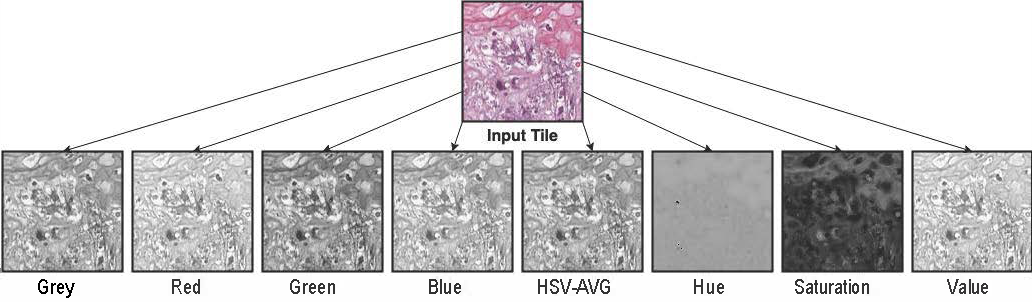
\includegraphics[width=\linewidth]{figures/RGB_HSV_channels.png}
    \caption{{\bf Eight Color Channels.} Different color channels are used to create sublevel filtrations. The figure is adapted from~\cite{yadav2023histopathological}.    \label{fig:color_channels}}
    \vspace{-.1in}
\end{wrapfigure}
Recall that for a given image $X$ with $r \times s$ resolution, the first step is to create a filtration, which is a nested sequence of binary images ${X_n}$. A common method to create such a sequence is to use the color values $\gamma_{ij}$ of each pixel $\Delta_{ij} \subset X$. Specifically, for a sequence of grayscale values $(t_1 < t_2 < \dots < t_N)$, one obtains a nested sequence of binary images $X_1 \subset X_2 \subset \dots \subset X_N$ such that $X_n = {\Delta_{ij} \subset X \mid \gamma_{ij} \leq t_n}$.




In~\cite{yadav2023histopathological}, the authors construct filtrations for cubical persistence by first extracting eight color channels $\gamma^k_{ij}$ from histopathological images with $1 \leq k \leq 8$, where each superscript $k$ corresponds to one color channel. The first four channels come from the RGB color space: red, green, blue, and grayscale (the average of R, G, and B). Additionally, they utilize the HSV color space, which includes hue, saturation, value, and their average (see~\Cref{fig:color_channels}). Each color channel defines a different filtration $\{\X_n^k\}_{n=1}^N$. In the paper, they set $N=100$.


\begin{figure}[t] 
	\centering
	\subfloat[\scriptsize Colon (Gray Betti-0) \label{fig:colon1}]{
	      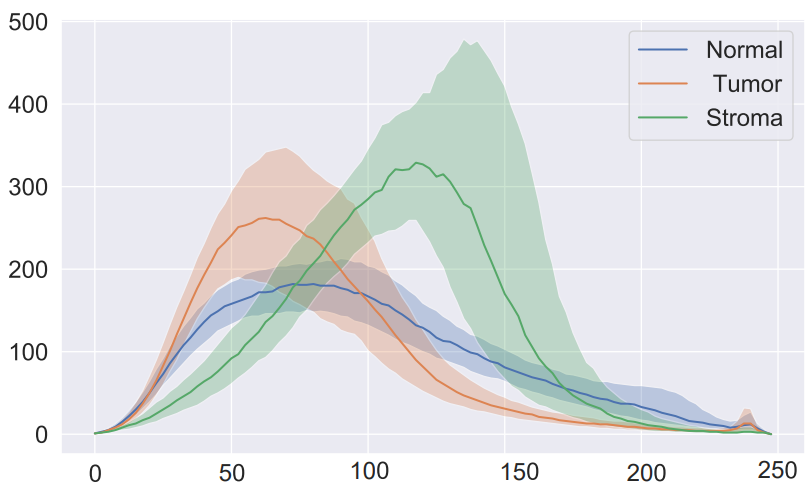
\includegraphics[width=0.33\linewidth]{figures/Colon_Gray_B0.PNG}}
	\subfloat[\scriptsize Bone (Gray Betti-0) \label{fig:bone1}]{
		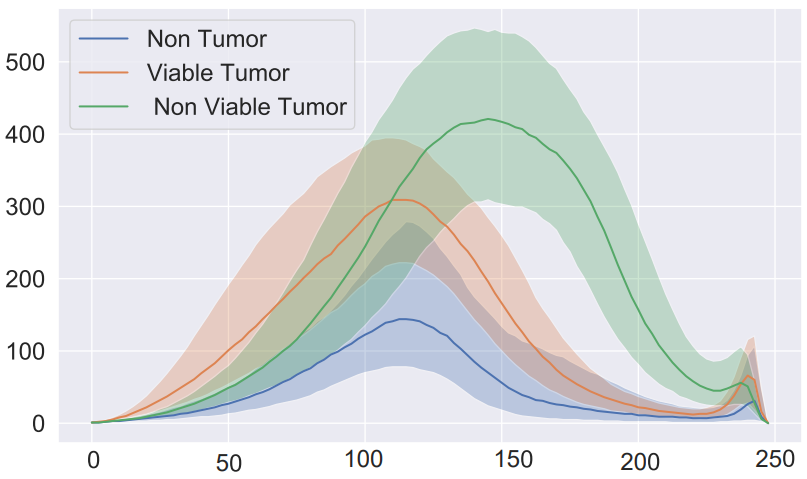
\includegraphics[width=0.33\linewidth]{figures/Bone_Gray_B0.PNG}}
	\subfloat[\scriptsize Cervical (Value Betti-0) \label{fig:cervical0}]{
		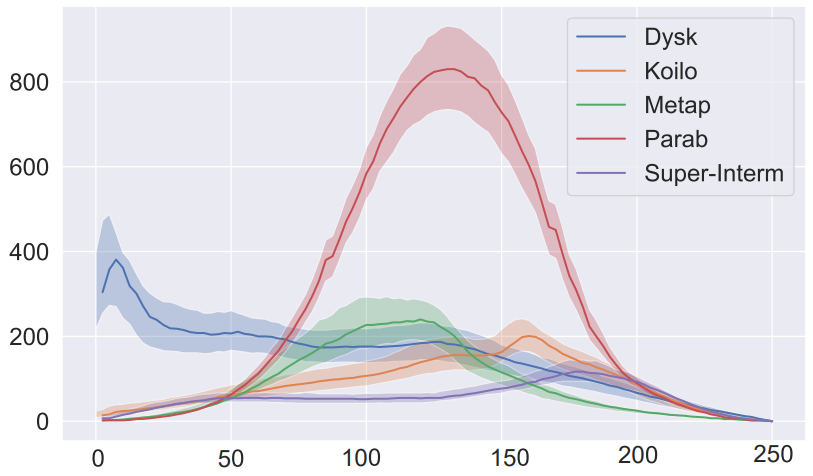
\includegraphics[width=0.33\linewidth]{figures/Cervical_Value_B0.PNG}}
	\caption{Median curves and 40\% confidence bands of Betti vectors, one for each cancer type.  $x$-axis represents color values $t\in[0,255]$ and $y$-axis represents $\beta_0(t)$ (Betti-0), i.e., the count of components in the binary image $\X_t$. For details, see~\cite{yadav2023histopathological}.}
	\label{fig:Betti-curves}
 \vspace{-.15in}
\end{figure}
Next, by using these filtrations, they obtain the corresponding persistence diagrams for dimensions $0$ and $1$. Then, by applying Betti vectorization to these persistence diagrams, they obtain $100$-dimensional Betti vectors $\vec{\beta}^k_m=[\beta^k_m(t_1) \dots \beta^k_m(t_{100})]$ where $k$ represents the color, and $m=0,1$ represents the dimension. Hence, $\beta^k_0(t_n)$ is the number of components (Betti-$0$ number) in the binary image $\X^k_n$, and $\beta^k_1(t_n)$ is the number of holes (Betti-$1$ number) in the binary image $\X^k_n$. Considering that there are eight color channels and two dimensions, one obtains 1600-dimensional vector $\vec{\beta}(\X)$ by concatenating these 16 vectors $\{\vec{\beta}^k_m\}$. By extracting extra features by utilizing local binary patterns (LBP) and Gabor filters, they produced another 800 and 400 dimensional features for each image, respectively. Then, they obtain a 2800-dimensional final vector $\wh{\beta}(\X)$. In particular, one can consider this as an image embedding method, and each image is realized as a point in $\R^{2800}$. Next, to improve the performance by removing correlated features, they use a feature selection method for the downstream task and reduce the vector size to 500 dimensions. 

They studied five cancer types, namely bone, breast, cervical, prostate, and colon cancer. In \Cref{fig:Betti-curves}, they provide the median curves and confidence bands for each class for three cancer types. As discussed earlier, while Betti vectors are considered as a weak vectorization method in general, they can be highly effective when the signature comes from the quantity and distribution of small features like these histopathological images. They utilized benchmark datasets for each cancer type consisting of 20K to 60K histopathological images. In~\Cref{tab:histopathology}, we give their results for various sets of feature vectors. Their results indicate that utilizing filtrations with multiple color channels can significantly improve the classification results in some cancer types, e.g., bone, breast, and colon cancers.



\begin{table}[h!]
\centering
\caption{{\bf Cancer diagnosis with PH.} Multiclass accuracy results for various cancer types from histopathological images using a topological ML model with a random forest classifier applied to different feature vector sets. The number of classes is indicated in parentheses. The first five rows correspond to the performance of Betti vectors across different color channels~\cite{yadav2023histopathological}. \label{tab:histopathology}}
\setlength\tabcolsep{3pt}
\begin{tabular}{lcccccc}
\toprule
\textbf{Features} & \textbf{\# Features} &  \textbf{Bone} (3) &   \textbf{Breast} (4)&   \textbf{Prostate} (4)&   \textbf{Cervical} (5)&   \textbf{Colon} (3)\\
    \midrule
Gray & 200               	&	84.6	&	68.8	&	91.1	&	54.6	&	 95.9 \\	
G-RGB & 800               	&	89.4	&	80.0	&	93.2	&	77.5	&	 97.5 \\	
avg HSV &200            	&	82.3	&	60.8	&	84.5	&	60.7	&	 88.0 \\	
HSV+ avg HSV & 800         	&	90.1	&	78.7	&	93.0	&	82.7	&	 97.5 \\	
All Betti features &1600 	&	90.8	&	82.8	&	93.9	&	85.5	&	 97.8  \\	
Betti + Gabor + LBP & 2800       	&	93.7	&	88.4	&	94.7	&	\textbf{92.6}	&	 \textbf{98.5} \\ \midrule	
Feature Selection  & 500    &	\textbf{94.2}	&	\textbf{91.6}	&	\textbf{95.2}	&	91.4	&	 98.4 \\ \bottomrule	
\end{tabular}
\end{table}








\subsection{Multiparameter Persistence: Computer Aided Drug Discovery} \label{sec:drug}

 

In this part, we outline an effective application of multiparameter persistence in computer-aided drug discovery (CADD), showcasing its use within the graph setting. For an application in the context of point clouds, see~\cite{vipond2021multiparameter, carriere2020multiparameter, loiseaux2024stable}.

Virtual screening (VS), a key technique in CADD, is used to identify potential drug candidates from a vast library of compounds that are most likely to bind to a specific molecular target. Demir et al.~\cite{demir2022todd} employed a multiparameter persistence approach for virtual screening by framing it as a graph classification task. In this method, compounds are represented as graphs, with atoms as nodes and bonds as edges. They adopted a ligand-based approach, wherein a few positive samples are provided for a given protein target, and the goal is to screen the compound library to find compounds that are most similar to these positive samples. Essentially, this approach can be viewed as a topology-based graph ranking problem. While their approach is more technical, here we outline the key concepts of their method. 




 \begin{wrapfigure}{r}{0.25\textwidth} 
    \vspace{-0.3cm}
  \begin{center}
    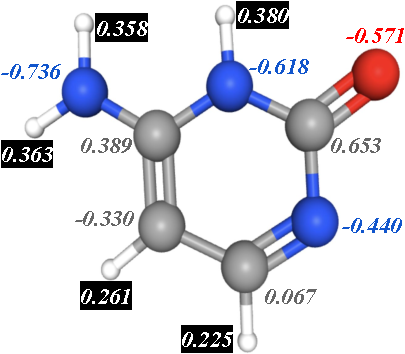
\includegraphics[width=\linewidth]{figures/cytosine.pdf}
    \caption{\footnotesize {\bf Cytosine}. Atom types are coded by their color: White=Hydrogen, Gray=Carbon, Blue=Nitrogen, and Red=Oxygen. The decimal numbers next to atoms represent their partial charges. The figure is adapted from~\cite{demir2022todd}.}
    \label{fig:cytosine}
  \end{center}
  \vspace{-0.5cm}
\end{wrapfigure} 

Their framework, TODD, generates fingerprints of compounds as multidimensional vectors (tensors), represented as a $2D$ or $3D$ array for each compound. The core idea is to simultaneously employ 2 or 3 highly relevant functions or weights (e.g., atomic mass, partial charge, bond type, electron affinity, distance) to obtain a multifiltration, which decomposes the original compound into substructures using these relevant chemical functions. As detailed in~\Cref{sec:MP-graph}, for a given compound $\G=(\V,\E)$, they used atomic number $A$ and partial charge $P$ as node functions $A:\V\to\R$ and $P:\V\to\R$, as well as bond strength $B$ as an edge function $B:\E\to\R$, to define multifiltrations. An illustration of such a multifiltration for the compound cytosine~\Cref{fig:cytosine} is provided in~\Cref{fig:MP-sublevel}. In this example, the functions are partial charge and atomic number. 
 


\begin{figure}[b]
\vspace{-.1in}
\centering
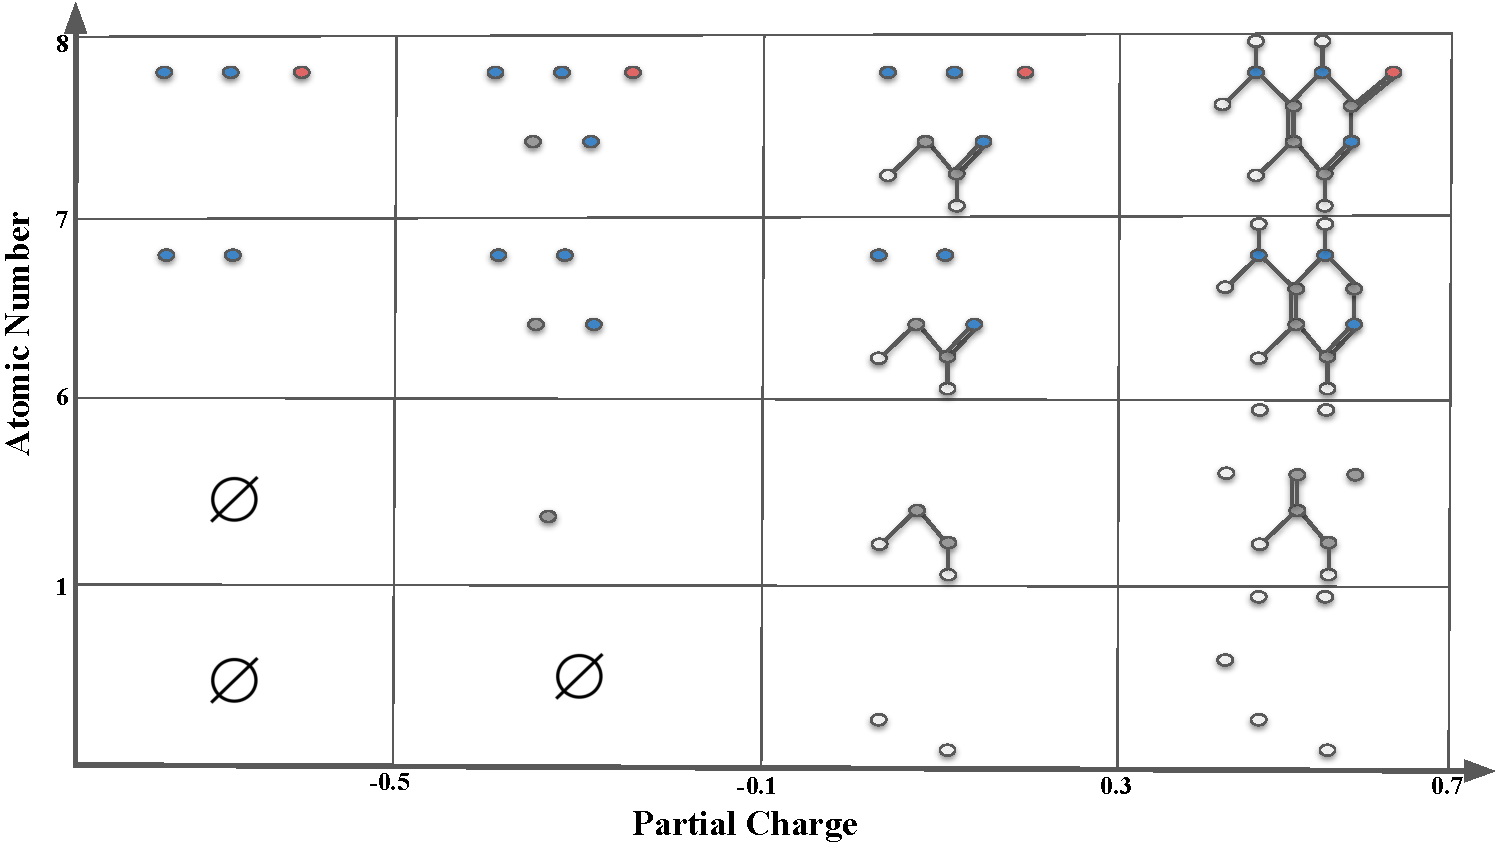
\includegraphics[width=0.8\textwidth]{figures/mp_persistence.pdf}
\caption{\footnotesize \textbf{Sublevel bifiltration of cytosine} is induced by filtering functions atomic charge $f$ and atomic number $g$. In the horizontal direction, thresholds $\alpha=-0.5,-0.1, +0.3,+0.7$ filters the compound into substructures $f(v)\leq \alpha$ with respect to their partial charge. In the vertical direction, thresholds $\beta=1,6,7, 8$ filters the compound in the substructures $g(v)\leq \beta$ with respect to atomic numbers. The figure is adapted from~\cite{demir2022todd}.} 
\label{fig:MP-sublevel}
\end{figure}
 
After constructing multifiltrations, they obtained compound fingerprints using a slicing technique. In particular, within each multifiltration ${\wh{\G}{ij}}$, they took horizontal slices by fixing a row $i_0$ to get a single persistence filtration ${\wh{\G}{i_0j}}$. For each horizontal slice $i_0$, they then generated a persistence diagram $\PD_k({\wh{\G}{i_0j}})$. These persistence diagrams were vectorized using Betti and Silhouette vectorizations to produce 2D arrays, such as $\mathbf{M}\beta=[\beta(\wh{\G}{ij})]$ (Betti numbers of the clique complex $\wh{\G}{ij}$).  



Next, using these 2D arrays, they applied two ML classifiers: Random Forest and ConvNeXt Vision Transformers. Both classifiers performed exceptionally well, surpassing all state-of-the-art models on benchmark datasets. In~\Cref{tab:todd2}, their results are shown for the DUD-E Diverse dataset, which comprises 116K compounds targeting eight proteins. The common metric in virtual screening is \textit{enrichment factor}, which compares the proportion of active compounds found in the top-ranked subset of a model output to the proportion of active compounds in the entire dataset. $EF_{1\%}$   represents the enrichment factor for the top $1\%$ of the dataset. 

 
 


\begin{table*}[t]
\centering
\caption{\footnotesize {\bf TODD vs. SOTA.} EF 1\% performance comparison between ToDD and the top-performing method among 12 SOTA baseline methods on eight targets from the DUD-E Diverse subset. \label{tab:todd2}}
\setlength\tabcolsep{4.5 pt}
\footnotesize
\begin{tabular}{lccccccccc}
\toprule
\textbf{Model} & \textbf{AMPC} &\textbf{CXCR4} & \textbf{KIF11} &\textbf{CP3A4} &\textbf{GCR} &\textbf{AKT1} &\textbf{HIVRT} &\textbf{HIVPR} &\textbf{Avg.}\\
\midrule
Best Baseline & 39.6 & 61.1 & 54.3 & 44.3 & 40.9 & 89.4 & 43.8 & 65.7 & 47.9 \\
\textbf{ToDD} &42.9 & 92.3 & 75.0  & 67.6 & 78.9 & 90.7  & 64.1  & 92.1 & 73.7 \\
\midrule
Relative gains & 8.3\% & 51.1\% & 38.1\% & 52.6\% & 92.9\%& 1.5\% & 46.3\% & 40.2\% & 52.8\% \\
\bottomrule
\end{tabular}
\end{table*}



\begin{figure}[b]
\centering
    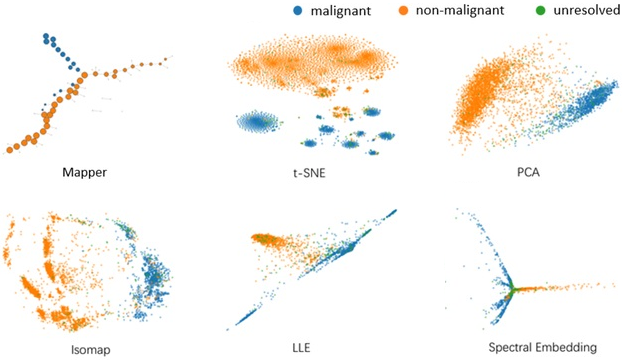
\includegraphics[width=0.8\textwidth]{figures/mapper1.png}
    \caption{{\bf Visualization Methods}. Visualization of melanoma cells in the expression space with different dimension reduction algorithms. The figure is adapted from~\cite{wang2018topological}. \label{fig:mapper}}
\end{figure}



\subsection{Mapper: Cancer Genotyping from RNA Sequencing} \label{sec:mapper-app}

In this section, we will explore a significant application domain for the Mapper algorithm: the analysis of single-cell RNA sequencing data. Recall that Mapper is particularly effective for analyzing high-dimensional point clouds by generating a low-dimensional graph summary that preserves local relationships (\Cref{sec:mapper}). In the Mapper summary graph, the nodes represent clusters in the point cloud, and the edges between the nodes indicate that the corresponding clusters are nearby (interacting) in the high-dimensional space.



RNA sequencing data is crucial for cancer genotype analysis, though it presents significant challenges. The expression profile of a cell can be mathematically represented as a point in a high-dimensional expression space, where each dimension corresponds to the RNA level of a gene, and the dimension of the space is the number of expressed genes. Points that are close to each other in this space correspond to cells with similar expression profiles. The set of all possible tumors of a cancer type spans a subspace of the expression space. From an ML perspective, this is a highly sparse point cloud in a high-dimensional space. In general, cells are assigned to some cancer subtype (e.g., malignant, benign, etc.), and the aim is to understand the relation of these types in this high-dimensional space. 


\begin{figure}[t]
\centering
    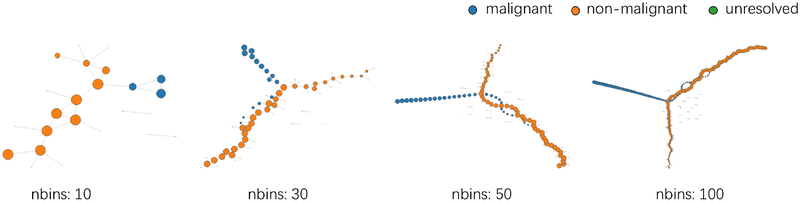
\includegraphics[width=0.8\textwidth]{figures/mapper-bins.jpg}
    \caption{\textbf{Mapper Graph for Varying Bin Sizes.} As the number of bins increases, the clusters become smaller, resulting in an increased number of nodes (clusters). The figure is adapted from~\cite{wang2018topological}. \label{fig:mapper-bin}}
\end{figure}



\begin{wrapfigure}{r}{3in}
\vspace{-.15in}
\centering
    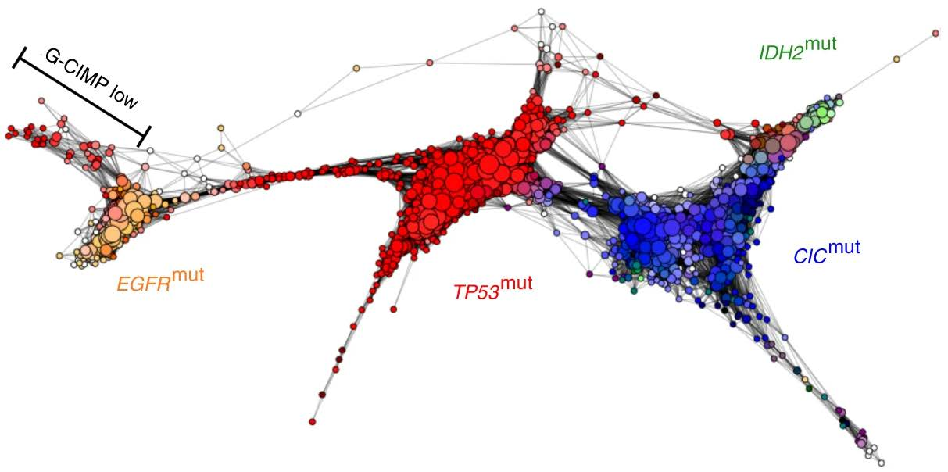
\includegraphics[width=\linewidth]{figures/mapper2b.pdf}
    \caption{\textbf{Genetic Alterations.} Topological representation of the expression space for low-grade gliomas using Mapper. The structure reveals three main clusters corresponding to distinct glioma subtypes. One cluster, labeled IDH2\textsuperscript{mut}, highlights the significance of the IDH2 gene in differentiating this subtype. This visualization emphasizes the distinct expression profiles that separate these glioma subtypes. This figure is adapted from~\cite{rabadan2020identification}.\label{fig:mapper-genetic}}
\end{wrapfigure}
There are several significant works on cancer genotyping through the use of Mapper techniques~\cite{rabadan2020identification,rizvi2017single,rafique2020topological}. In this paper, we will detail the methods in two works. In the first one~\cite{wang2018topological}, Wang et al. conducted a comparative analysis of Mapper visualization techniques on RNA-sequencing data. They used the melanoma tumor cells dataset GSE72056, which contains 4,645 cells. Of these, 1,257 are malignant, and 3,256 are non-malignant, with some minority classes included. The dataset includes 23,686 expressed genes. From an ML perspective, this data can be represented as a point cloud $\X = \{x^i\}_{i=1}^{4645}$ in very high dimensional space $\R^{23,686}$, where each dimension corresponds to a gene $\{\gamma_j\}_{j=1}^{23,686}$. In particular, for a cell $x^i \in \X$ with $x^i = (x^i_1, x^i_2, \dots, x^i_{23,686})$, $x^i_j$ represents the RNA level of gene $\gamma_j$ in cell $x^i$. This is computed as $x^i_j = \log_2\left(1 + \frac{\text{TPM}_{ij}}{10}\right)$, where $\text{TPM}_{ij}$ is the transcript-per-million (TPM) for gene $\gamma_j$ in cell $x^i$. Notice that the number of dimensions far exceeds the number of points. From an ML perspective, this presents a highly challenging setup. In~\Cref{fig:mapper}, the authors illustrate different dimension reduction techniques on this dataset. In~\Cref{fig:mapper-bin}, they show how the graph changes when the number of bins (resolution) is varied. 


In the second work~\cite{rabadan2020identification}, Rabadan et al. applied the Mapper algorithm to identify somatic mutations relevant to tumor progression. They analyzed mutation and RNA expression data for 4500 genes across 4476 patients from 12 tumor types, including low-grade glioma (LGG), lung adenocarcinoma, breast invasive carcinoma, and colorectal adenocarcinoma. This study led to the identification of 95 mutated cancer genes, 38 of which were previously unreported. They identified three large expression groups with oligodendrogliomas (enriched for CIC and IDH2 mutations), IDH1-mutant astrocytomas (enriched for TP53 mutations), and IDH1-wild-type astrocytomas (enriched for EGFR mutations)~(\Cref{fig:mapper-genetic}). In their analysis, they used the neighborhood lens (\Cref{sec:mapper}) as the filter function and scanned the resolution and gain parameter space to determine the optimal parameters~(\Cref{fig:mapper-bin}).  










